\section{Results}
In the following sections results will be presented for the AMPL implementation and for both of the heuristics. The parameter values used in the runs will also be presented. 

\subsection{AMPL implementation}\label{sec:ampl_res}

Implementing the model in AMPL and running the model in CPLEX 12.5 gives the resulting values for the three objective function components displayed in Table \ref{tab:CPLEX_res}. The weights in equations \ref{objfcn} and \ref{constr:s_min} were set to $L = 2$, $A = 1$, $M =100$ and $N=1$, thus making librarians twice as valuable as assistants and stand ins 100 times more valuable than no shift changes. 

\begin{table}[!h]
\centering
\caption{Results from running the Mathematical Model in CPLEX.}
\label{tab:CPLEX_res}
\begin{tabular}{|l|p{3cm}|p{3cm}|l|}
\hline
\rowcolor{Gray} & \textbf{Min num stand ins (lib, ass)} & \textbf{AMPL stand-in cost} & \textbf{Solution time} \\ \hline
\cellcolor{Gray} \textbf{Result} & \multicolumn{1}{c|}{(3,0)} & \multicolumn{1}{c|}{6} & \multicolumn{1}{c|}{19 min} \\
\hline
\end{tabular}
\end{table}

These results can be used as benchmark in the heuristics as CPLEX returns an optimal solution. 

\subsection{Week block scheduling approach}
As most of the costs are correlated with each other some parameter tuning has been required. The final result of the parameter tuning can be seen in Table \ref{tab:cost_parameters}. Their respective descriptions can be seen in Table \ref{tab:all_costs}. 

\begin{table}[!h]
\centering
\caption{List of all costs used in week block scheduling approach and their respective values.}
\label{tab:cost_parameters}
\begin{tabular}{|c|c|}
\hline
\rowcolor[HTML]{FD6864} 
\multicolumn{2}{|l|}{\cellcolor{corn} \textbf{Demand costs}} \\ \hline
%\multicolumn{2}{|c|}{\cellcolor[HTML]{FD6864}Demand costs}    \\ \hline
\rowcolor[HTML]{C0C0C0} 
Cost name                                      & Cost value       \\ \hline
Demand\_few\_ass                        & 350         \\ \hline
Demand\_few\_lib                        & 300         \\ \hline
Demand\_many\_ass                       & 200         \\ \hline
Demand\_many\_lib                       & 40          \\ \hline
Demand\_few\_total                             & 800         \\ \hline
Demand\_many\_total                            & 700         \\ \hline
Demand\_evening\_cost         & 20,000 				\\ \hline
Demand\_PL\_good\_ass        & 1,200            \\ \hline
Demand\_PL\_good\_lib        & 800           \\ \hline
Demand\_PL\_bad\_ass         & 1,200           \\ \hline
Demand\_PL\_bad\_lib         & 1,600             \\ \hline
\rowcolor[HTML]{FD6864} 
\multicolumn{2}{|l|}{\cellcolor{corn} \textbf{PL amount costs}} \\ \hline
\rowcolor[HTML]{C0C0C0} 
Cost name                                      & Cost value       \\ \hline
PL\_good\_amount                  & 1,000                   \\ \hline
PL\_violate\_amount             & 1,500                  \\ \hline
\rowcolor[HTML]{FD6864} 
\multicolumn{2}{|l|}{\cellcolor{corn} \textbf{Weekend costs}} \\ \hline
\rowcolor[HTML]{C0C0C0} 
Cost name                                      & Cost value       \\ \hline
HB\_amount                       & 15,000    \\ \hline
No\_weekend                & 5,000                   \\ \hline
\rowcolor[HTML]{FD6864} 
\multicolumn{2}{|l|}{\cellcolor{corn} \textbf{Stand-in costs}} \\ \hline
\rowcolor[HTML]{C0C0C0} 
Cost name                                      & Cost value       \\ \hline
Stand\_in\_cost                     & 5     \\ \hline
\end{tabular}
\end{table}

Worth noting is that these values are most certainly not optimal as they have mostly been assigned using intuition. However, a few relations were determined by either running some tests or using reason. An example is either if $PL\_good\_cost > Demand\_PL\_good\_ass$ or $PL\_good\_cost > Demand\_PL\_good\_lib$. If so, all workers that can be assigned another PL will be, leaving the library overstaffed with PL workers. The reason is because the net of $-PL\_good\_cost + Demand\_PL\_good\_ass/lib$ will be negative meaning it is a preferable insertion even though the library will be overstaffed.

Table \ref{successful_iter} shows the amount of successful iterations on a run. This run is using the same cost parameters shown in Table \ref{tab:cost_parameters}. 
\begin{table}[!h]
\centering
\caption{Amount of successful iterations}
\label{successful_iter}
\begin{tabular}{|c|c|}
\hline
Successful iterations         & 420      \\ \hline
Iterations (total) & 638      \\ \hline
\%                 & $\sim$66 \\ \hline
\end{tabular}
\end{table}

Based on the same data as in Table \ref{successful_iter} the average stand-in value per iteration can be calculated. It is seen in Table \ref{tab:average_stand_ins}.
\begin{table}[!h]
\centering
\caption{Average stand-in value per iteration}
\label{tab:average_stand_ins}
\begin{tabular}{|c|c|}
\hline
Stand-in value & 105      \\ \hline
Number of iterations         & 420      \\ \hline
Average stand-in value      & 0.25 \\ \hline
\end{tabular}
\end{table}
A librarian is multiplied by a factor two and an assistant is multiplied by a factor one.

Having an average stand-in value of 0.25 means that most of the times no stand-ins are found. Table \ref{tab:stand_in_spread} shows statistics of how many stand-ins were found after 420 successful iterations. 
\begin{table}[!h]
\centering
\caption{Amount of stand-ins found after 420 successful iterations.}
\label{tab:stand_in_spread}
\begin{tabular}{|c|c|}
\hline
\rowcolor[HTML]{D2D2D2} 
Stand-in spread & Times \\ \hline
No stand-ins    & 351                      \\ \hline
1 assistant     & 33                      \\ \hline
1 librarian 	& 36 \\ \hline
\end{tabular}
\end{table}

Figure \ref{fig:feasibleRerun} shows a plot of the objective function value after destroy and repair iterations. When the value on the y-axis reaches zero, a solution is found. Every time the value skyrockets a solution has been discarded and a new iteration starts. This is done until a solution is found. 

%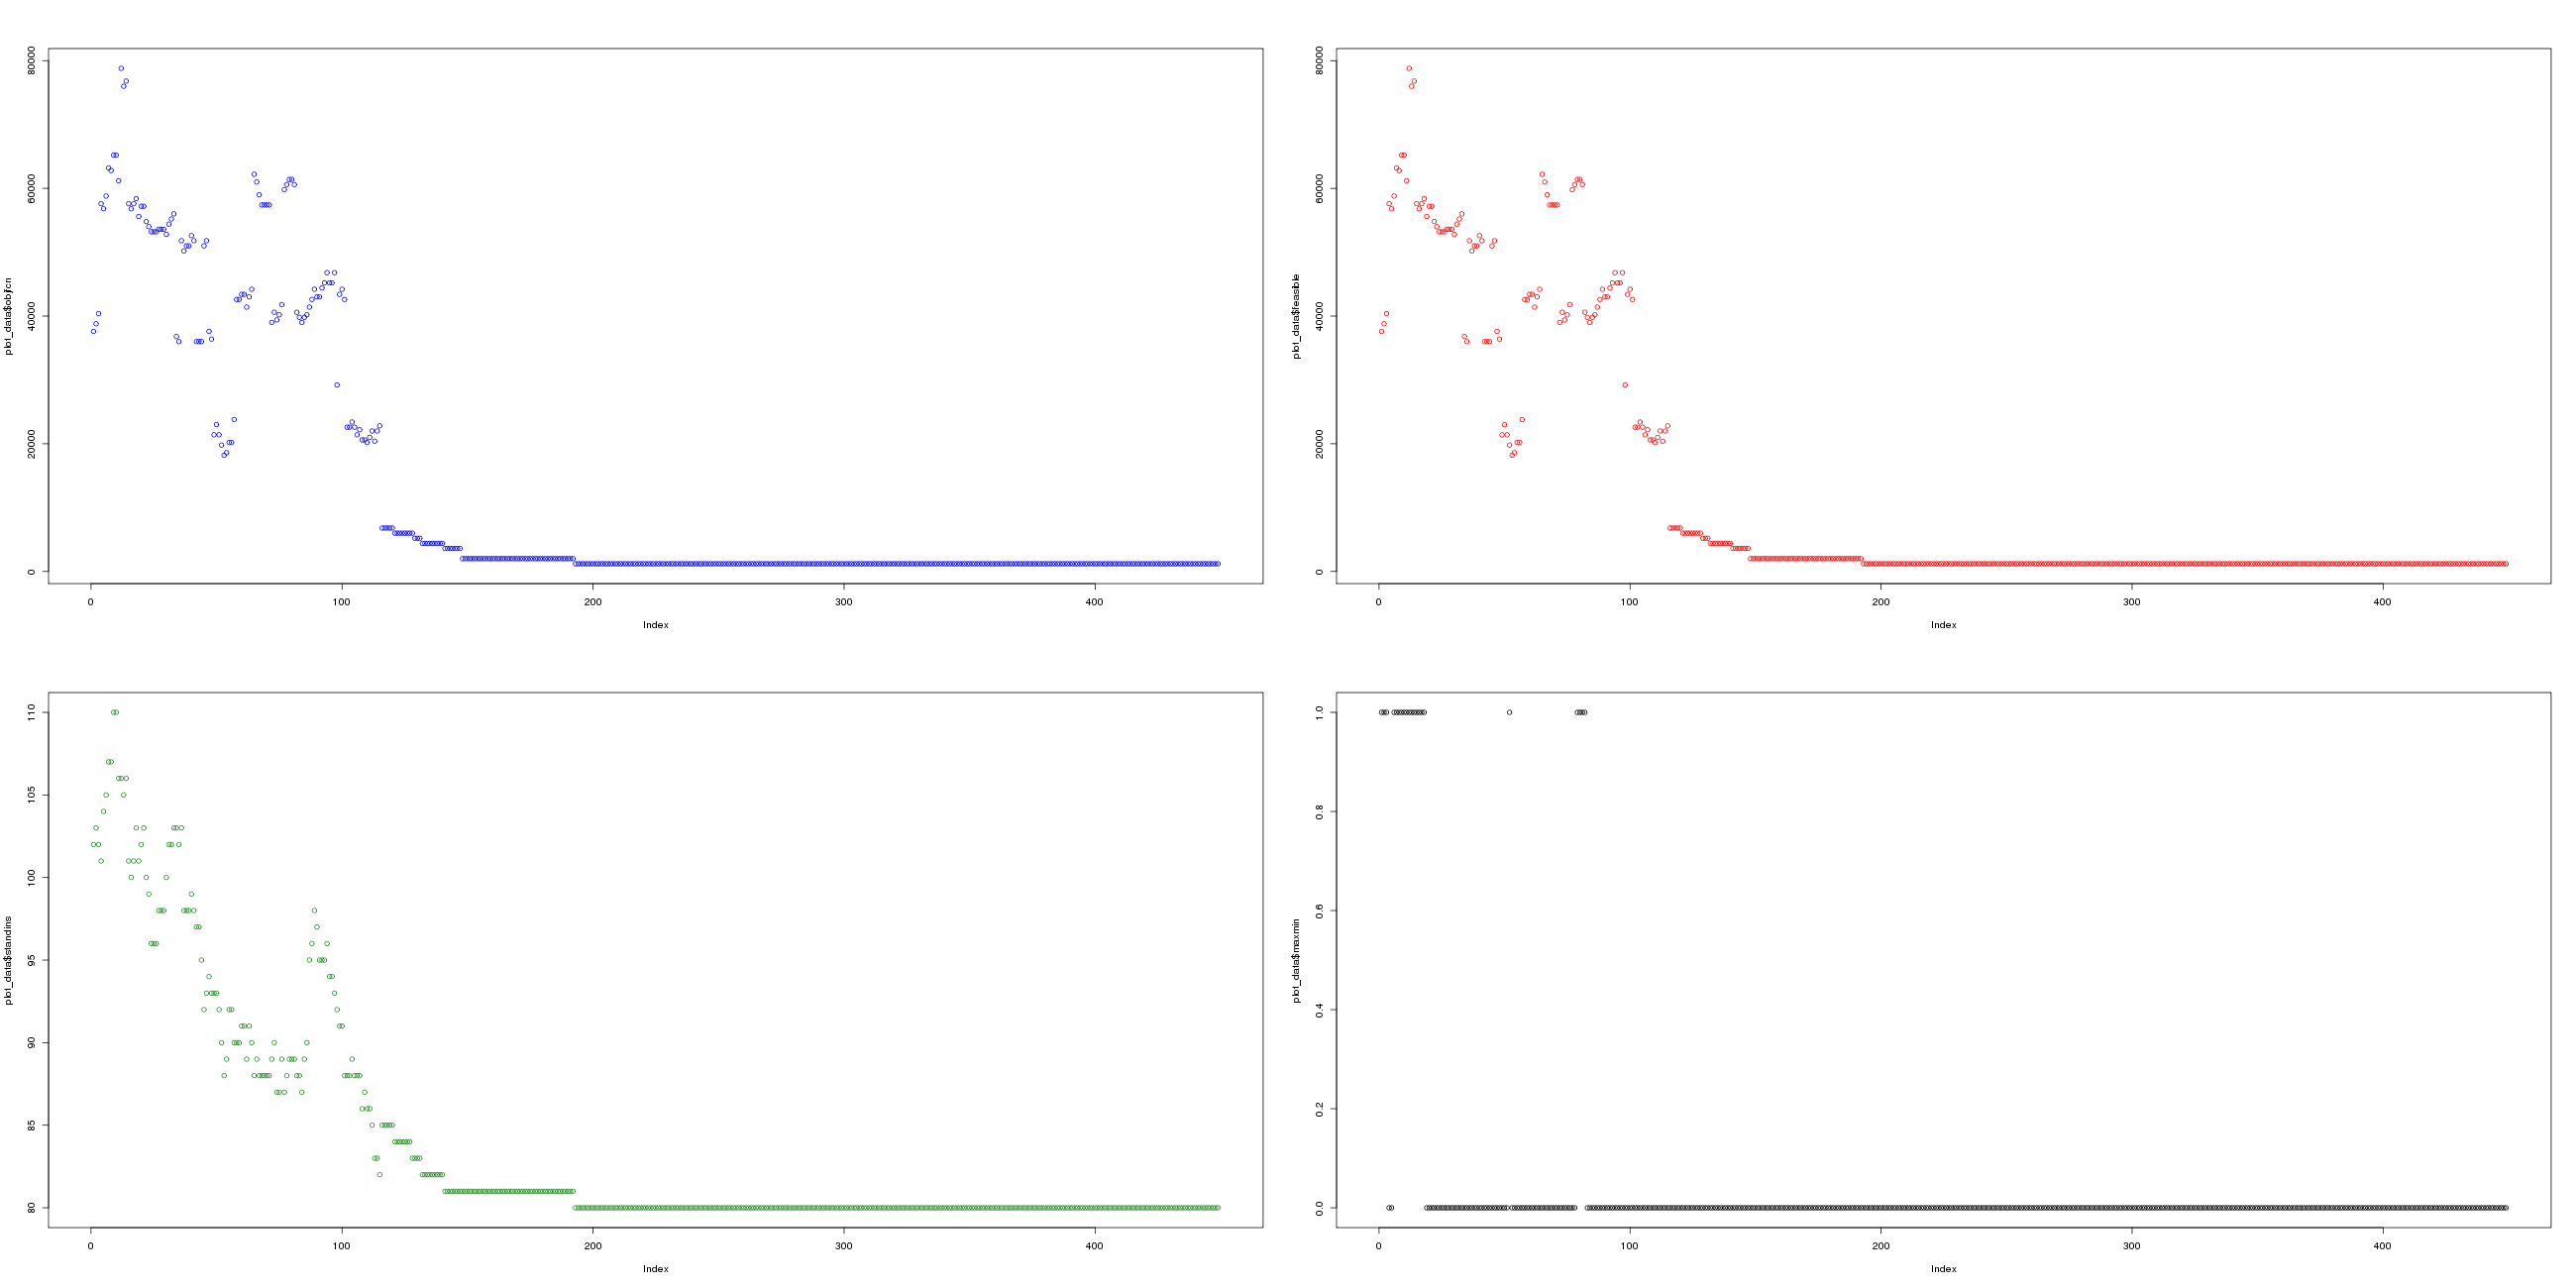
\includegraphics[scale = 0.3, width = 15cm]{Rplot}
%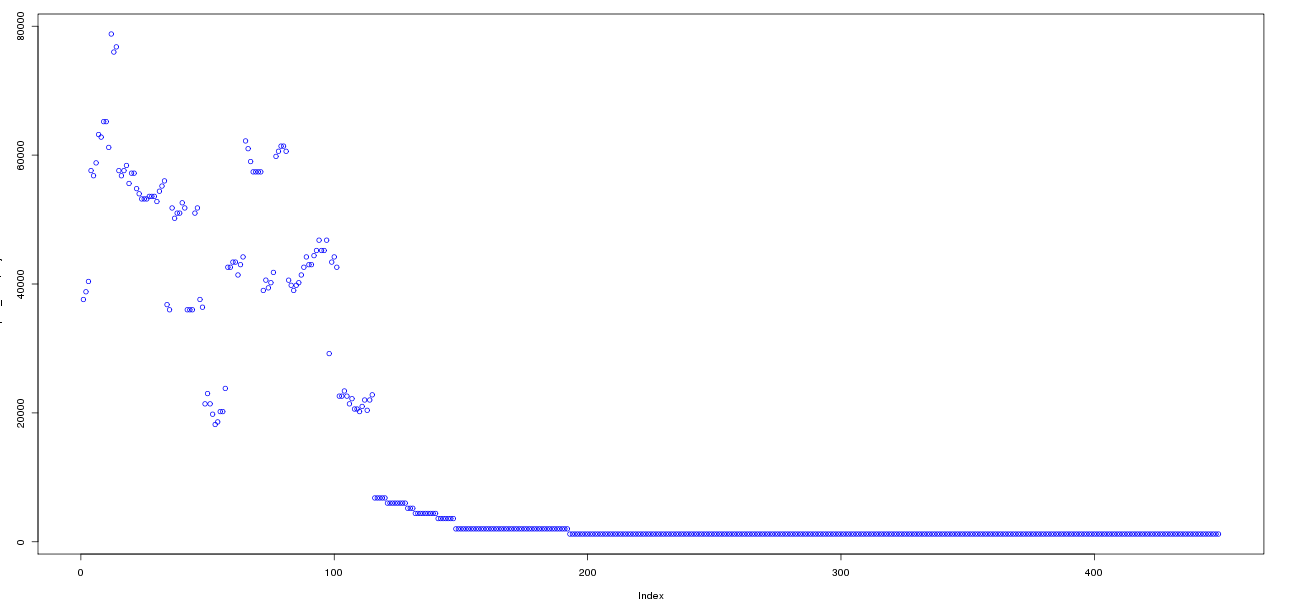
\includegraphics[scale = 0.3, width = 15cm]{1Plot}
\begin{figure}[!h]
\centering
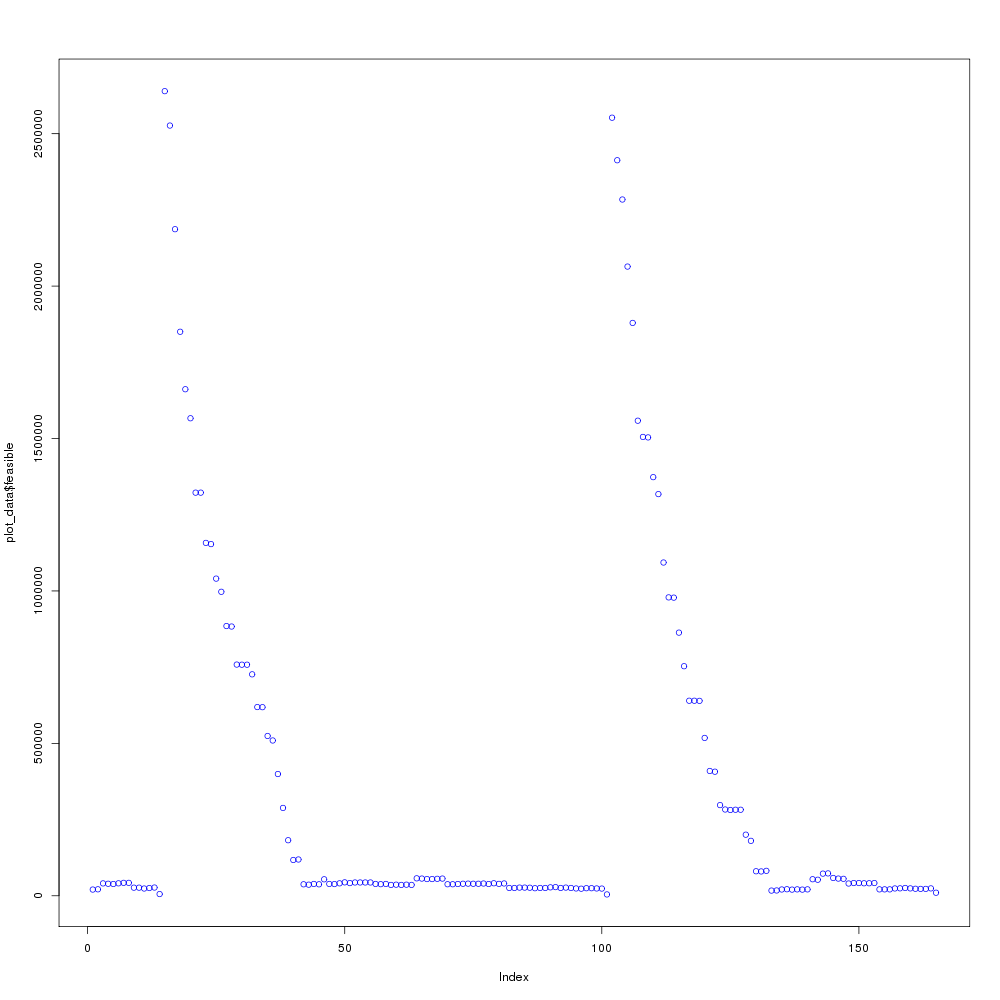
\includegraphics[scale = 0.3]{Chapters/ImagesClaes/Rfeasible.png}
\caption{Plot of the objective function value after every new destroy and repair iteration.}
\label{fig:feasibleRerun}
\end{figure}

\subsection{Task distribution approach}\label{sec:task_dist_res}

In order to find a good value for the weights described in Section \ref{section:tasks_cost}, different tuning tests were performed. These tests resulted in the weights presented in Table \ref{tab:tasks_weight}. These weights are used in all test in this section unless stated otherwise. 

\begin{table}[!h]
\centering
\caption{Weights used in the implementation.}
\label{tab:tasks_weight}
\begin{tabular}{|l|l|}
\hline
\rowcolor{gray!90} \textbf{Weight} & \textbf{Weight value} \\ \hline
\multicolumn{2}{|l|}{\cellcolor{Gray} \textbf{Weekend Objective Function Weights}} \\ \hline
$W_{SI\_m}$ & 0.1 \\ \hline
$W_{S\_m}$ & 0.1 \\ \hline
$W_{D\_m}$ & 10 \\ \hline
$W_{SI\_a}$ & 0.01 \\ \hline
$W_{S\_a}$ & 0.01 \\ \hline
$W_{D\_a}$ & 1 \\ \hline
\multicolumn{2}{|l|}{\cellcolor{Gray} \textbf{Worker/Worker Objective Function Weights}} \\ \hline
$W_{w\_SI}$ & 
\begin{tabular} [x]{@{}c@{}}
	2 \text{if librarian} \\ 
	1 \text{if assistant}
\end{tabular} \\ \hline
$W_{Task\_D}$ / $W_{w\_Task\_D}$ & 100\\ \hline
$W_{Task\_W}$ / $W_{w\_Task\_W}$ & 	10 \\ \hline
$W_{PL\_W}$ / $W_{w\_PL\_W}$ & 5 \\ \hline
$W_{PL\_Tot}$ / $W_{w\_PL\_Tot}$ & 5 \\ \hline
$W_{SShift\_W}$ / $W_{w\_SShift\_W}$ & 4 \\ \hline
\end{tabular}
\end{table}



The first six weights, belonging to the weekend objective function, were most experimented with and will be discussed further in this section. The first three, the min weights, are scaled relatively to each other, while the latter three are simple calculated as one tenth of their equivalent min weights. The weights in Equation \ref{eq:wend_cost_calc}, $W_{lib}$ and $W_{ass}$ were set to $2$ and $1$ respectively since it can be argued that one librarian can perform twice as many tasks as one assistant.

The individual worker cost and the worker objective function costs measuring the same aspect of the schedule have been given the same weights, as is illustrated in Table \ref{tab:tasks_weight}. This is due to the fact that the weights, relative to each other, decide what constraints are most strict. It is, for example more severe to break the rule of one task per day, than to break the rule of having too many shifts at the same time in a week, which is reflected in the weights. The stand-in weight $W_{w\_SI}$ is twice as high for librarians as for assistant.

It was argued in Chapter \ref{chap:taskdist} that the critical part of the problem is the weekend placement, which is why a two-phase algorithm was implemented. Both phases are run a specified number of iterations, referred to as $It_{wend}$ and $It_{wday}$. These parameters were also trimmed and the results from different iteration values are displayed in Tables \ref{tab:taskdist_res_wendit} and \ref{tab:taskdist_res_wdayit}. The results for weight tuning are displayed in Table \ref{tab:taskdist_weights_res}.

\begin{table}[!h]
\centering
\caption{Results from the task distribution heuristic when varying $It_{wend}$}
\label{tab:taskdist_res_wendit}
\begin{tabular}{|l|l|l|}
\hline
\rowcolor{Gray} \textbf{$It_{wend}/It_{wday}$} &  \textbf{Heuristic cost} &  \textbf{AMPL cost} \\ \hline
\cellcolor{Gray} \textbf{10/10} & \multicolumn{1}{c|}{4.40} & \multicolumn{1}{c|}{4.78} \\
\cellcolor{Gray} \textbf{50/10} & \multicolumn{1}{c|}{5.00} & \multicolumn{1}{c|}{5.34} \\
\cellcolor{Gray} \textbf{100/10} & \multicolumn{1}{c|}{5.26} & \multicolumn{1}{c|}{5.52} \\
\cellcolor{Gray} \textbf{500/10} & \multicolumn{1}{c|}{5.66} & \multicolumn{1}{c|}{5.78} \\
\cellcolor{Gray} \textbf{1000/10} & \multicolumn{1}{c|}{5.54} & \multicolumn{1}{c|}{5.66}  \\
\hline
\end{tabular}
\end{table}

\begin{table}[!h]
\centering
\caption{Results from the task distribution heuristic when varying $It_{wday}$}
\label{tab:taskdist_res_wdayit}
\begin{tabular}{|l|l|l|}
\hline
\rowcolor{Gray} \textbf{$It_{wend}/It_{wday}$} &  \textbf{Heuristic cost} &  \textbf{AMPL cost} \\ \hline
\cellcolor{Gray} \textbf{500/5} & \multicolumn{1}{c|}{5.47} & \multicolumn{1}{c|}{5.74} \\
\cellcolor{Gray} \textbf{500/10} & \multicolumn{1}{c|}{5.66} & \multicolumn{1}{c|}{5.78} \\
\cellcolor{Gray} \textbf{500/15} & \multicolumn{1}{c|}{5.6} & \multicolumn{1}{c|}{5.74} \\
\cellcolor{Gray} \textbf{500/20} & \multicolumn{1}{c|}{5.57} & \multicolumn{1}{c|}{5.74} \\
\hline
\end{tabular}
\end{table}


\begin{table}[!h]
\centering
\caption{Results from the task distribution heuristic when varying weights. $It_{wend} = 1000$ and $It_{wday} = 20$ in all runs.}
\label{tab:taskdist_weights_res}
\begin{tabular}{|l|l|l|}
\hline
\rowcolor{Gray} \textbf{$W_{SI\_m}/W_{S\_m}/W_{D\_m}$} & \textbf{Heuristic cost} &  \textbf{AMPL cost} \\ \hline
\cellcolor{Gray} 0/0/0 & \multicolumn{1}{c|}{2.85} & \multicolumn{1}{c|}{3.66}  \\
\cellcolor{Gray} 1/1/1 & \multicolumn{1}{c|}{5.43} & \multicolumn{1}{c|}{5.54}  \\
\cellcolor{Gray} 10/0.1/0.1 & \multicolumn{1}{c|}{5.11} & \multicolumn{1}{c|}{5.36}  \\
\cellcolor{Gray} 0.1/10/0.1 & \multicolumn{1}{c|}{5.43} & \multicolumn{1}{c|}{5.60}  \\
\cellcolor{Gray} 0.1/0.1/10 & \multicolumn{1}{c|}{5.57} & \multicolumn{1}{c|}{5.80} \\
\hline
\end{tabular}
\end{table}

The tables display two costs for each test, the Heuristic cost and the AMPL cost. These are calculated as the average result of 100 runs. The heuristic cost is the actual result of the heuristic, measuring how good the heuristic solves the problem, while the AMPL cost is the result obtained when solving the problem to optimality in CPLEX, using the weekends found in the heuristic. Thus, this value measures how good the weekend phase works. Both figures should be compared to the optimal stand-in value for the problem, which is 6 (Table \ref{tab:CPLEX_res}).

Studying Table \ref{tab:taskdist_res_wendit}, it can be seen that the AMPL cost increases with more weekend iterations. However, after 500 iterations, the cost stops to improve and it is actually deteriorating. This is probably indicating that the weekend objective function value can only give a measure of a good schedule, thus the result does not only depend on the number of iterations but also on chance. 

Similarly, in Table \ref{tab:taskdist_res_wdayit}, the Heuristic cost increases until a certain threshold, when the solutions are not improving any more. This might indicate that the second phase is not varied enough, so the same schedules are found many times. This might be solved through varying weights or introducing more randomness in task placement.

Table \ref{tab:taskdist_weights_res} shows a few extreme weight combinations. It is is clear from the table that although the performance does not vary to any larger extent when shifting the focus in the weights, using a completely random search with no weights produces bad results. The last combination of weights seems to be performing slightly better than the others and thus, these weights were chosen as optimal weights.

The weekend objective function value during a typical run is shown in Figure \ref{fig:obj_fun_vals}. The effects of the SA accept function are visible in the plot as smaller or larger dives in the objective function value. In the measuring, the SA-parameters $T_0 = 0.4$ and $\alpha = 0.985$. $It_{wend} = 1000$ were used. The graph suggests that a high weekend objective function value is found already within the 200 first iterations, which is consistent with the results in Table \ref{tab:taskdist_res_wendit}.

\begin{figure}[!htbp]
\centering
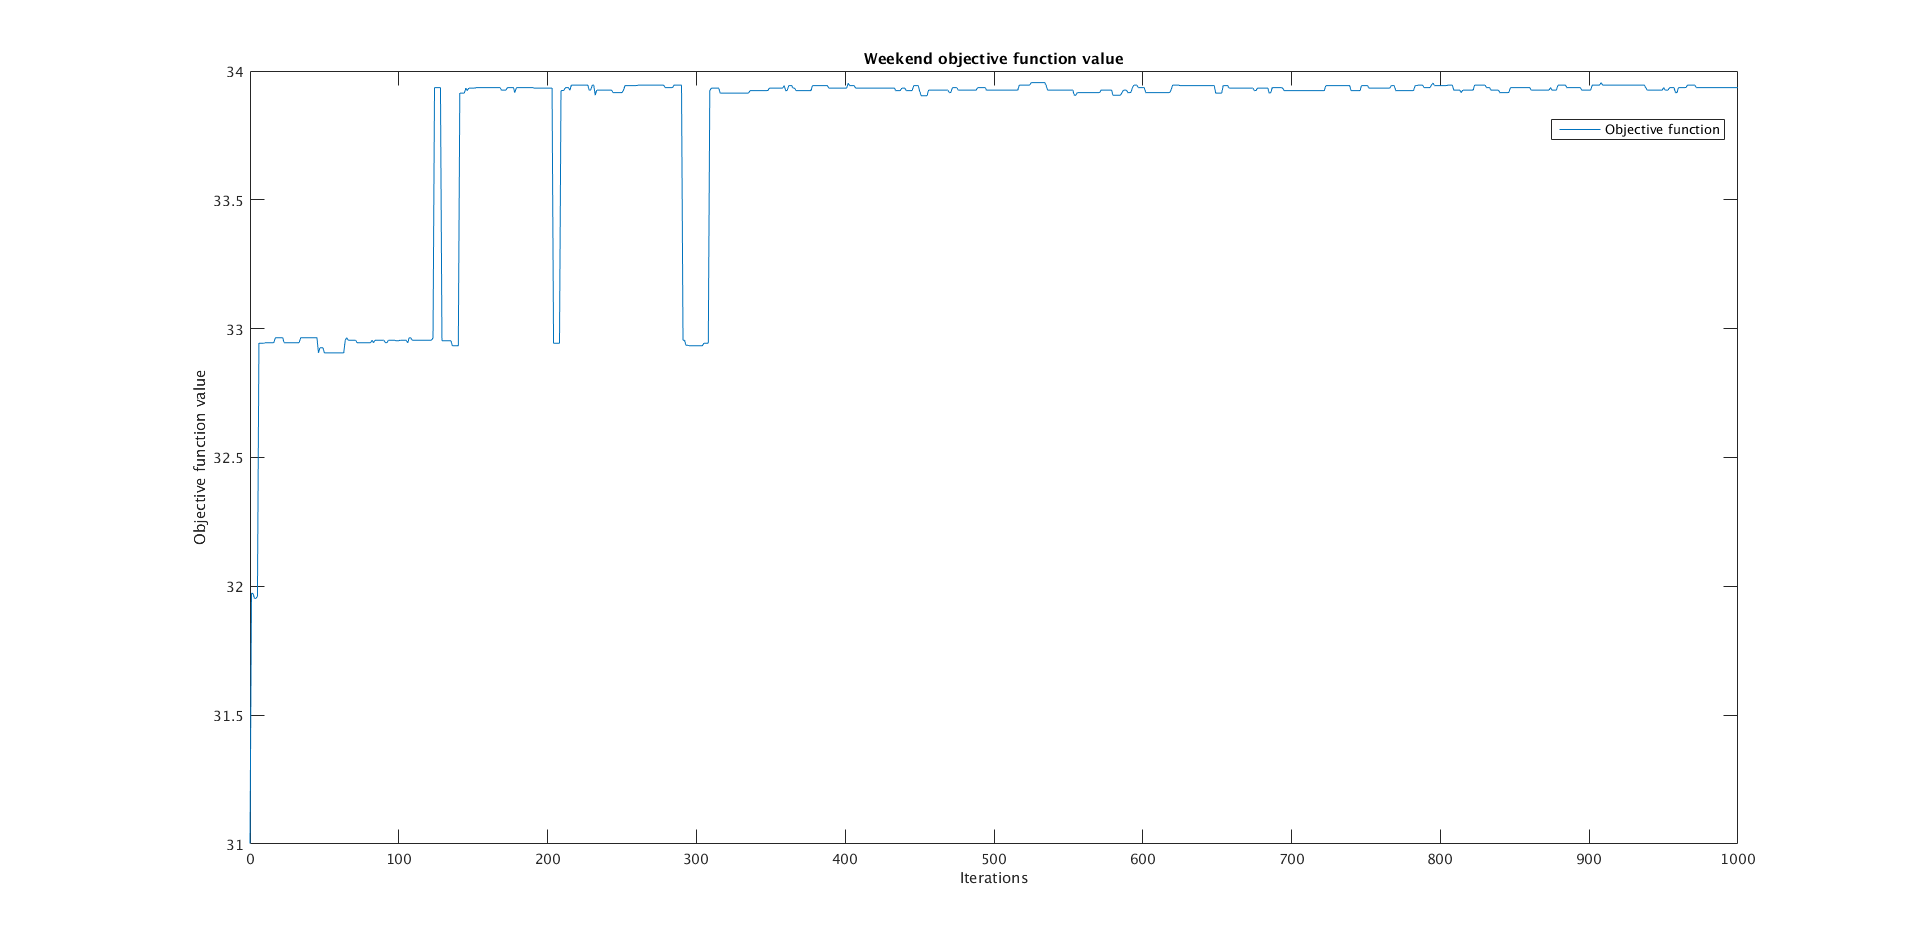
\includegraphics[width=0.9\textwidth, trim = 100px 0px 100px 20px, clip]{Chapters/ImagesEmelie/Plot_1000_20.png}
\caption{The weekend objective function for 1000 iterations}
\label{fig:obj_fun_vals}
\end{figure}


\begin{figure}[!htbp]
\centering
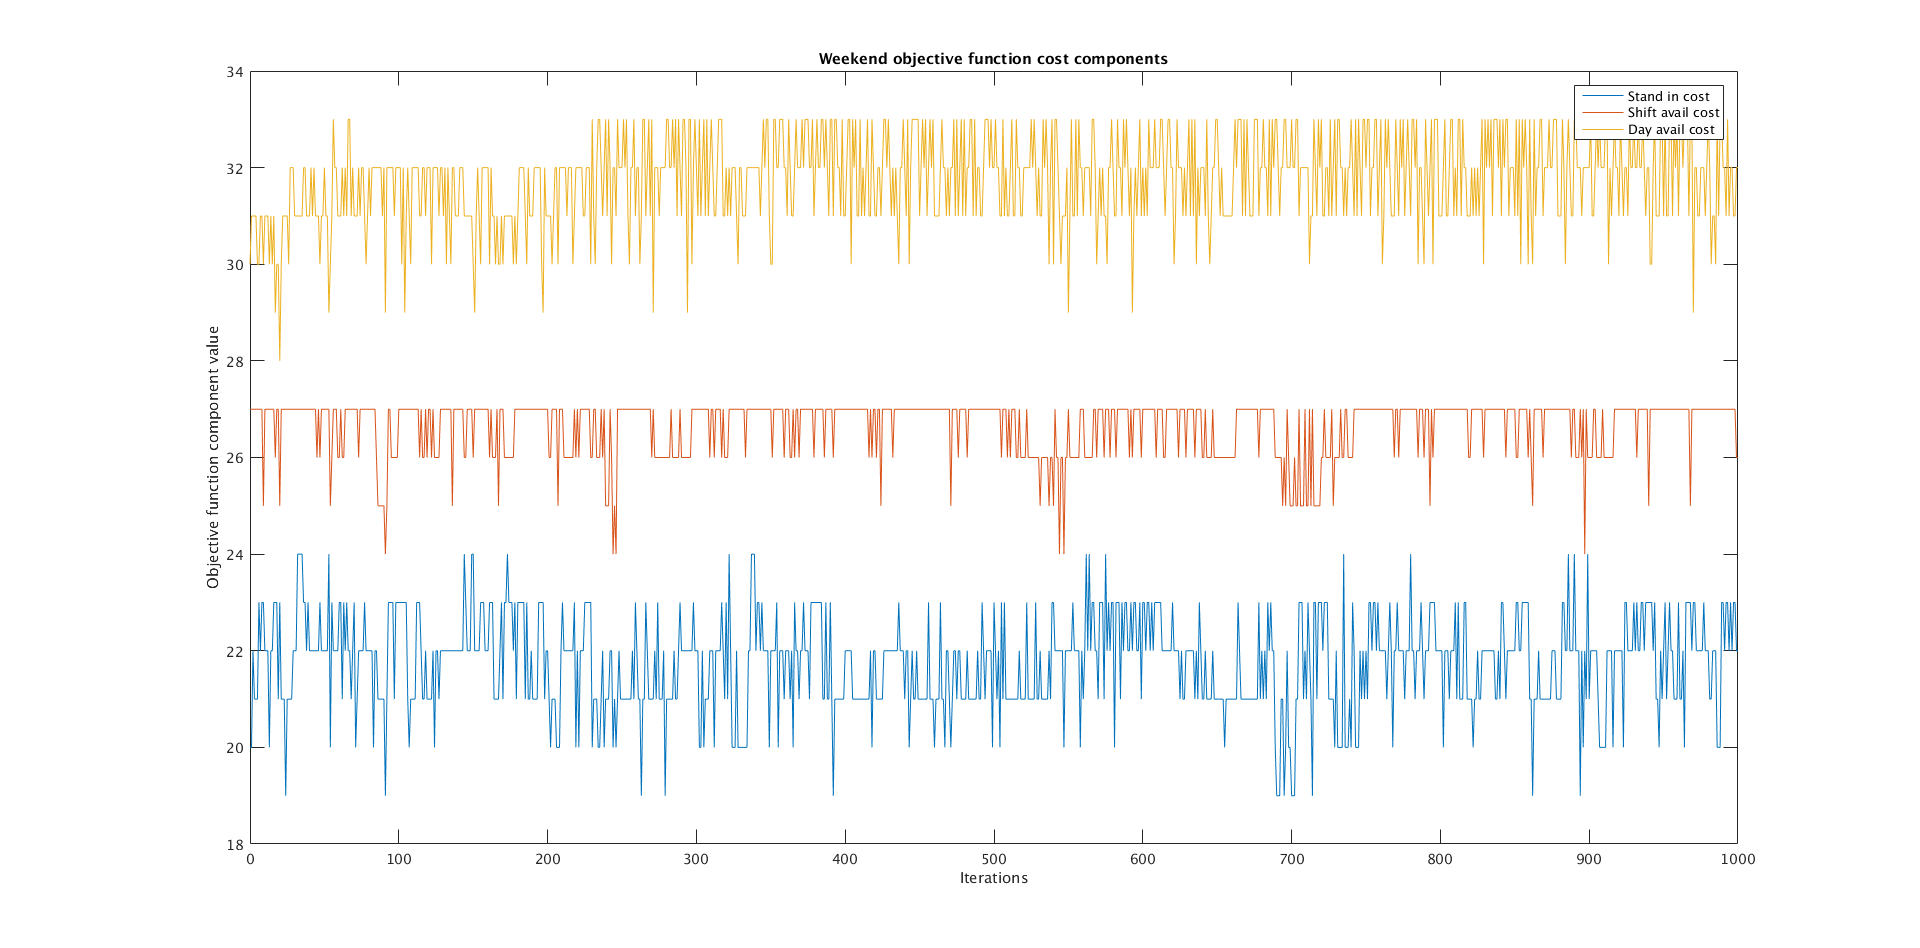
\includegraphics[width=0.9\textwidth, trim = 100px 0px 100px 20px, clip]{Chapters/ImagesEmelie/Components_1000_20.png}
\caption{The weekend objective function minimum cost components for 1000 iterations}
\label{fig:obj_fun_comp}
\end{figure}

\begin{figure}[!h]
\centering
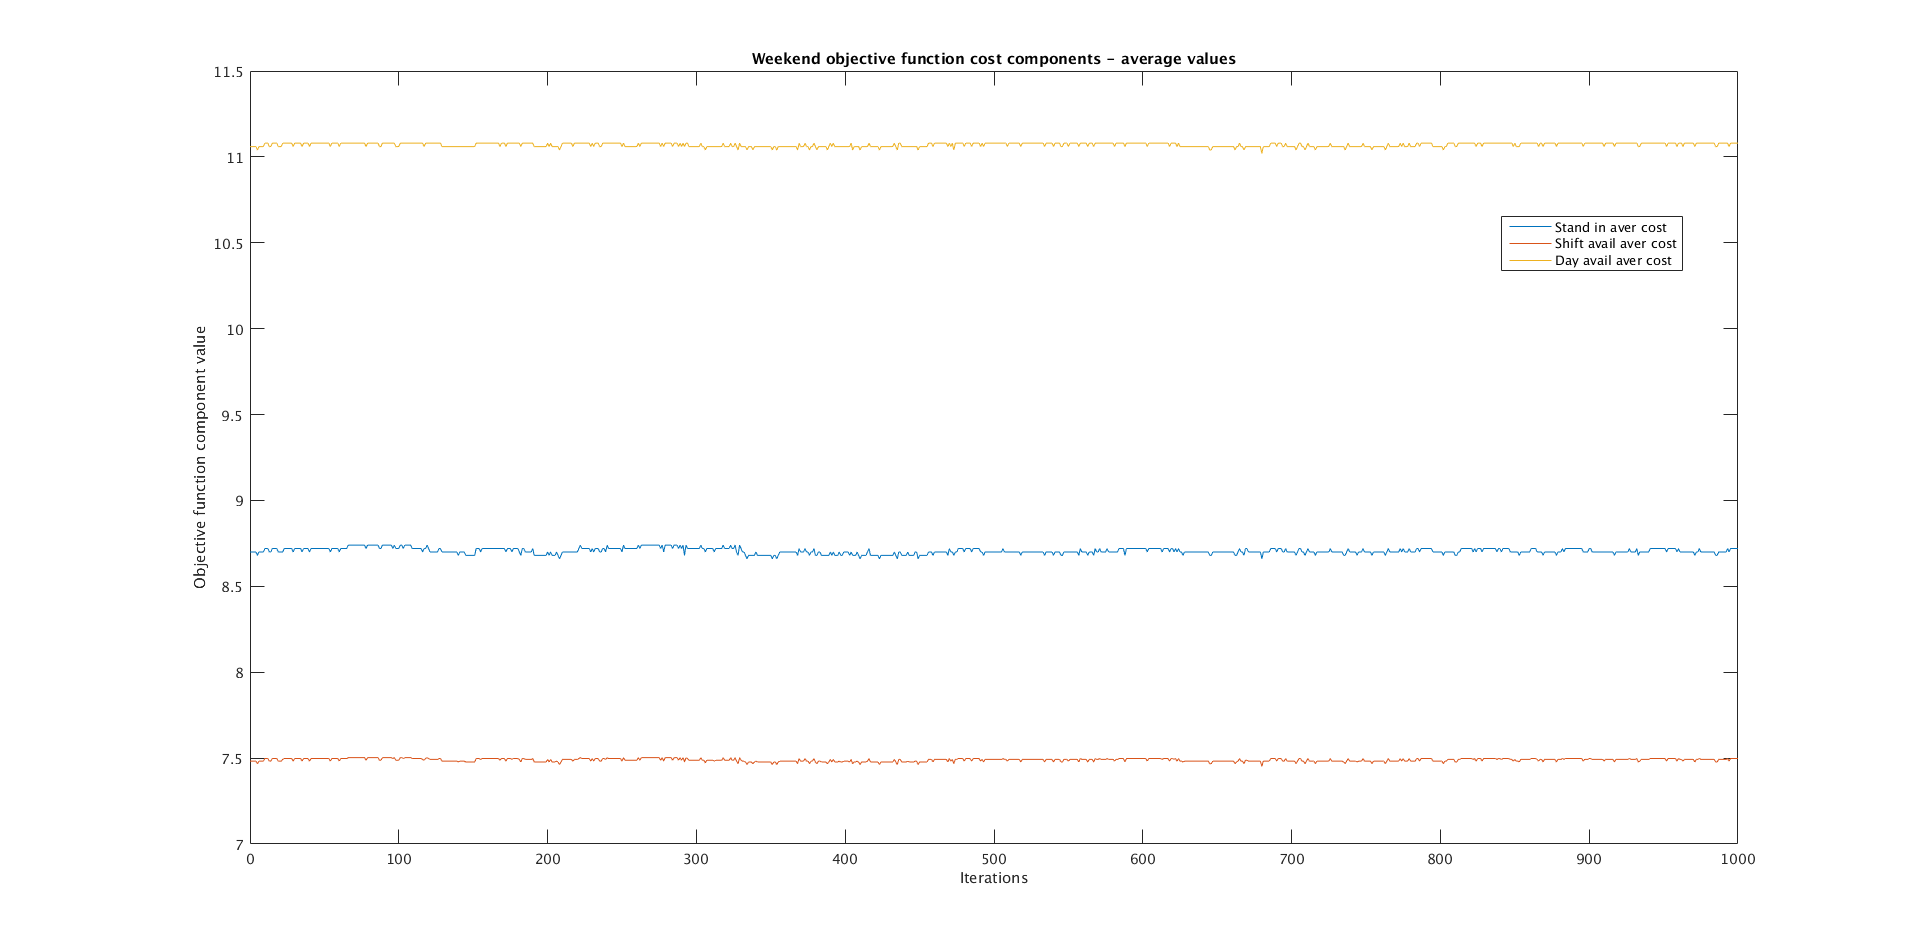
\includegraphics[width=0.9\textwidth, trim = 100px 0px 100px 20px, clip]{Chapters/ImagesEmelie/Components_av_1000_20.png}
\caption{The weekend objective function average costs components for 1000 iterations}
\label{fig:obj_fun_comp_aver}
\end{figure}


In Figure \ref{fig:obj_fun_comp} and Figure \ref{fig:obj_fun_comp_aver}, the three different cost components from the weekend objective function for the same run are displayed. In the first plot, the minimum costs are displayed. These seem to fluctuate between a few discrete values, although a small improvement the iterations can be seen at least in the day avail cost component. The average values are almost constant throughout the iterations, as can be seen in the second plot. This is probably due to the fact that the total number of workers barely changes when shifting their weeks.

Attempts were made to correlating the min components of the weekend objective function value. However, the results were fluctuating between different tests and no clear correlations could be identified. This suggests that they are measuring three independent aspects.

\section{Discussion}
In this Section, the different results from in the previous Section will be discussed. Pros and cons for both methods are also given so that they can be more easily compared.


\subsection{Week block scheduling approach}
Table \ref{tab:pros_cons_weekly_scheduling} lists pros and cons with the implemented week block scheduling approach. Some pros and cons were considered before the heuristic was chosen. Mainly the con concerning the exponential growth was taken into consideration as an estimation of the upper limit of the problem size was done. Also, the pro regarding the same amount of week blocks was taken into consideration, as the heuristic was thought of having firstly a block construction phase and secondly an assignment phase. 


 Weekends, solution time and costs are no major issues as they can be avoided by a few smarter implementations. For instance, weekends can be improved by assigning values when each worker is available on a day and from those numbers create an even distribution of possible stand-ins and therefore increase the lowest value of stand-ins through the days. This shall implicitly decrease the solution time as less iterations will be required. However, to always be able to create a pool of week appearances regardless of problem size can easily become a major issue. Just by adding meetings and the assignment of Library on Wheels tasks to the problem makes it grow considerably.

\begin{table}[H]
\caption{Pros and cons with the implemented week block scheduling approach}
\label{tab:pros_cons_weekly_scheduling}
\begin{tabularx}{\linewidth}{>{\parskip1ex}X@{\kern4\tabcolsep}>{\parskip1ex}X}
\toprule
\hfil\bfseries Pros
&
\hfil\bfseries Cons
\\\cmidrule(r{3\tabcolsep}){1-1}\cmidrule(l{-\tabcolsep}){2-2}

%% PROS, seperated by empty line or \par
The same amount of week block appearances will exist for five and ten weeks.\par
Quick iterations when destroying and repairing.\par

&

%% CONS, seperated by empty line or \par
Weekends needs to be assigned in a more systematically way in order to achieve reasonable results regarding lowest amount of stand-ins through the days.\par
The amount of unique block appearances grows exponentially in case more task types are added, such as meetings.\par
The solution time can vary considerably as several random generators have been used.\par
A great deal of costs are needed (some correlated), where each of them affects the solution procedure.

\\\bottomrule
\end{tabularx}
\end{table}

 

\subsection{Task distribution approach}
The results from the previous Section point to the fact that placing a good weekend structure is essential in order to get a good final schedule. When $It_{wend}$ is increased the results improve, up to a limit around 500 iterations where the results are comparable to those of the AMPL implementation. This suggests that the weekend objective function used gives an indication of a good schedule. However, this is only an indication, not a guarantee for an optimal solution as the results converge to a value slightly lower than the AMPL result. 

Table \ref{tab:taskdist_weights_res} suggests that the weights used in the weekend objective function are important to how well the implementation works, but only to a certain degree. More testing could be done on the weights in order to see if the result can be further improved. However, since the objective function is an incomplete measure of a good schedule the results will never be completely optimal. This is listed as the main drawback in the cons column in Table \ref{tab:pros_cons_task_scheduling}. 

\begin{table}[!ht]
\caption{Pros and cons with the implemented task distribution approach}
\label{tab:pros_cons_task_scheduling}
\begin{tabularx}{\linewidth}{>{\parskip1ex}X@{\kern4\tabcolsep}>{\parskip1ex}X}
\toprule
\hfil\bfseries Pros
&
\hfil\bfseries Cons
\\\cmidrule(r{3\tabcolsep}){1-1}\cmidrule(l{-\tabcolsep}){2-2}

%% PROS, seperated by empty line or \par
In most cases, the method finds the optimal solution. \par
The method is very fast compared to the CPLEX solver. Only a few iterations in each phase gives good results. \par
The method can be used to find a good weekend schedule. The rest of the schedule can then be placed using another method such as CPLEX. \par

&

%% CONS, seperated by empty line or \par
The weekend objective function is not an exact measurement of a good weekend schedule. \par


\\\bottomrule
\end{tabularx}
\end{table}

\iffalse
\begin{table}[!h]
\centering
\label{tab:taskdist_res}
\caption{Results from the task distribution heuristic. Weights from Table \ref{tab:tasks_weight}}
\begin{tabular}{|l|l|l|l|}
\hline
\rowcolor{Gray} \textbf{$It_{wend}/It_{wday}$} &  \textbf{Heuristic cost} &  \textbf{AMPL cost} & \textbf{$\rho_{O\_A}$} \\ \hline
\cellcolor{Gray} \textbf{100/20} & \multicolumn{1}{c|}{5.22} & \multicolumn{1}{c|}{5.48} & 0.58 \\
\cellcolor{Gray} \textbf{500/20} & \multicolumn{1}{c|}{5.64} & \multicolumn{1}{c|}{5.74} & -0.20 \\
\cellcolor{Gray} \textbf{1000/10} & \multicolumn{1}{c|}{5.54} & \multicolumn{1}{c|}{5.66} & 0.03 \\
\cellcolor{Gray} \textbf{1000/20} & \multicolumn{1}{c|}{5.57} & \multicolumn{1}{c|}{5.80} & 0.08 \\
\cellcolor{Gray} \textbf{1000/30} & \multicolumn{1}{c|}{5.50} & \multicolumn{1}{c|}{5.68} & -0.06 \\
\hline
\end{tabular}
\end{table}
\fi
